\documentclass[conference]{IEEEtran}
\IEEEoverridecommandlockouts
% The preceding line is only needed to identify funding in the first footnote. If that is unneeded, please comment it out.
\usepackage{cite}
\usepackage{amsmath,amssymb,amsfonts}
\usepackage{algorithmic}
\usepackage{graphicx}
\usepackage{textcomp}
\usepackage{float}
\usepackage{caption}
\usepackage{xcolor}

\def\BibTeX{{\rm B\kern-.05em{\sc i\kern-.025em b}\kern-.08em
    T\kern-.1667em\lower.7ex\hbox{E}\kern-.125emX}}
\begin{document}



\title{\textbf{Facial Keypoints Detection}\\
\vspace{0.29cm}
\large \\
\large \\
{\footnotesize \textsuperscript{}}
%\thanks{Identify applicable funding agency here. If none, delete this.}
}


\author
{\IEEEauthorblockN{\textsuperscript{}Luis Oliveros Colón}
\IEEEauthorblockA{\textit{Artificial Intelligence for ECE} \\
\textit{Stevens Institute of Technology}\\
NJ, USA \\
lolivero@stevens.edu}
\and
\IEEEauthorblockN{\textsuperscript{} Rucha Waghulde}
\IEEEauthorblockA{\textit{Artificial Intelligence for ECE} \\
\textit{Stevens Institute of Technology}\\
NJ, USA \\
rwaghuld@stevens.edu}
\and
\IEEEauthorblockN{\textsuperscript{} Siddharth Mandgi}
\IEEEauthorblockA{\textit{Applied Artificial Intelligence} \\
\textit{Stevens Institute of Technology}\\
NJ, USA \\
smandgi@stevens.edu}
}


\maketitle

\begin{abstract}
Facial Key Points Detection is an important and challenging problem in the fields of computer vision and machine learning. There is difficulty to catch keypoints on the face due to complex influences from original images, very different facial features from person to person and there is no guidance to suitable algorithms. It involves predicting the co-ordinates of the Facial Keypoints, e.g. nose tip, center of eyes, etc, for a given face. As the development of deep learning, more and more methods based on it are proposed for solving related issues, which bring numerous revolutionary changes.

In this project, we propose a simplified method based on Convolution Neural Network for solving the problem of detecting facial key points. We are given a list of 96×96-pixel 8- bit graylevel images with their corresponding (x, y) coordinates of 15 facial keypoints. We first locate the keypoints in each image using Deep Convolutional Neural Network algorithm. Our algorithm trains the facial keypoints data and assess its performance on the test set to evaluate predictions. 
\end{abstract}

\begin{IEEEkeywords}
Keypoints, facial images, LeNet, Convolutional Neural Networks
\end{IEEEkeywords}

\section{Introduction}
\subsection{Motivation}
Our primary motivation for this project was our interest in applying deep learning to significant problems with relevant uses. Facial recognition is a very popular biometric technique these days. Various developments have already been observed in facial recognition technologies, but there is still a huge scope and a need for improvement. We are excited about applying the applications of Facial Key Points Detection as a building block in several applications such as tracking faces in images and videos, Analysing Facial Expressions, Detecting Dysmorphic Facial Signs for Medical Diagnosis and Biometrics/ Face Recognition. The idea that we were working towards solving an open and important problem with all these possible applications greatly inspired us.

We specifically chose the Facial Keypoints Detection project because it will give us an opportunity to experiment with a wide variety of deep learning approaches, work with different neural networks and solve the problems associated with it.

The competition element also allowed us to benchmark our results against the greater community and compare the effectiveness of our methods against alternatives. Lastly, we were motivated by the inherent challenges associated with the problem. 

Detecting facial keypoints is a challenging problem given the variations in both facial features as well as image conditions. Facial features may differ according to size, position, pose and expression, while image quality may vary with illumination and viewing angle. These variations, in combination with the necessity for highly accurate coordinate predictions (e.g. the exact corner of an eye) have led us to believe that through this project we will be gaining insights about a deep and an interesting topic.


\subsection{Project Definition}
The goal of this project is to create an algorithm which can provide accurate prediction on the positions of the facial keypoints on face images. Our objective is to locate 15 sets of facial keypoints of eyes, eyebrows, nose and mouth, when given a raw facial image. We have used deep structures for facial keypoints detection, which can learn well from different faces and overcome the variance between faces of different person or of different conditions to a great extent. The algorithm which is used in this project is Deep Convolutional Neural Network. For the given images, we have applied Convolutional Neural Network to train our model with these images and then evaluate our predictions on the other images. As a result, we can see the actual and predicted keypoints on face images.

\subsection{Project Flow}


\textbf{Understanding the dataset:} In this dataset, we are provided with the training and testing data folders that contain face images with image data as row-ordered list of pixels and the coordinates for facial keypoints.
    
\textbf{Data Pre-processing:} This step involved importing the images and using their paths to access these images and apply different augmentation techniques. So, this data pre-processing step will include loading and reading the dataset and making it ready for training.
    
\textbf{Training:} For training, the algorithm used is Convolutional Neural Network (CNN). Other optimization algorithms like Adam or Stochastic Gradient Descent is be used to minimize the error associated with this data.
    
\textbf{Testing:} After training our model using CNN, we evaluate our predictions using the test dataset. This will let us know how our model will be training and decide on whether we should modify its structure or hyperparameters. Then we use this final trained model to predict facial keypoints on the images.



\section{Related Work}
This section consists of research work from several authors who have worked on detecting facial keypoints using different algorithms. Many of these researches from different authors have aided us in developing our project so far. 

Traditional methods have explored feature extraction strategies includes texture-based and shape-based features and different types of graphic models to detect facial keypoints.  

[1] proposed a method that uses Gabor wavelet feature based boosted classifiers which can detect 20 different facial keypoints with limited head rotation and different illumination conditions. [2] also use Gabor features for detecting facial keypoints. Using a sample log Gabor response of a facial point, the authors have shown that the locations on the test facial images that are like the sample facial points can be detected. [3] focused on keypoints detection for Textured 3D Face Recognition. Features are extracted by fitting a surface to the neighbourhood of a Keypoint and sampling it on a uniform grid. And then PCA are used for dimensional reduction and then projected and matched from a probe and gallery face.

Other methods have designed probability graphic models to capture the relationship between different pixels and features to detect facial keypoints. Using Markov Random Fields, [4] exploits the constellations that facial points can form. Also, the authors used boosted regression to learn the mappings from the pixel’s appearance of the area around the keypoints and the location of the keypoints. These models have reached high performance on aligned faces but still need improvements for faces under different environment conditions. [5] have proposed a model to detect the target location by local evidence aggregation. By aggregating the estimates obtained from stochastically selected local appearance information into a single robust prediction other than focus only on the target location only, the proposed model has solved the regression problem from a new prospective.

Recent works have focused on deep architectures for this detection task since these structures can better capture the high-level features of an image, in our problem a given face. [6] proposed a three-level carefully designed convolutional networks, which at first capture the global high-level features, and then refine the initialization to locate the positions of keypoints. On the other hand, [7] used pretrained DBN on surrounding feed-forward neural network with linear Gaussian output layer to detect facial keypoints. 

Recent works have focused on deep architectures for this detection task since these structures can better capture the high-level features of an image, in our problem a given face. [6] proposed a three-level carefully designed convolutional networks, which at first capture the global high-level features, and then refine the initialization to locate the positions of keypoints. On the other hand, [7] used pretrained DBN on surrounding feed-forward neural network with linear Gaussian output layer to detect facial keypoints. 

These researches have helped us understand the importance of detection of facial key points and challenges associated with it. Upon careful analysis of the different algorithms, we have realized the need to create an efficient model which would correctly predict the facial key points and ensure a highly accurate performance. 



%\includegraphics[scale=0.54]{Table.png}
 
\section{Implementation}

This project is done in various stages illustrated in the project flow. We have used a deep learning python library; PyTorch to implement this project code. Our Project was Implemented on Google Collab and its GPU aided in optimizing and accelerating our deep learning frameworks. 

\subsection{Dataset Description}
We have used the dataset from Kaggle Competition – Facial Key Points Detection. There are 15 Facial Keypoints per face image like left eye center, right eye center, left eye inner corner, left eye outer corner, right eye inner corner, right eye outer corner, left eyebrow inner end, left eyebrow outer end, right eyebrow inner end, right eyebrow outer end, nose tip, mouth left corner, mouth right corner, mouth center top lip and mouth center bottom lip (Fig.1). 

\begin{figure}[h!]
    \centering
    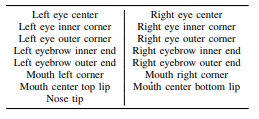
\includegraphics[scale=1.0]{keypoints.png}
    \caption{15 Facial Keypoints}
    \label{fig:my_label}
\end{figure}

Our data set consists of a list of 7049 two-dimensional 8-bit graylevel training images with their corresponding (x, y) coordinates of the 15 facial keypoints. Each input image is represented by a size of 96 × 96 pixel, with pixel values in range of [0, 255]. The given training set is a huge matrix of size 7049 × 31, where each row corresponds to one image, the first 30 target columns give the (x, y) values for each of the 15 facial keypoints, and each entry in the last column is a long list of 9216 numbers representing the pixel matrix of each image melted row by row.


In some examples, some of the target keypoint positions are missing (encoded as missing entries in the csv, i.e., with nothing between two commas).

The test dataset consists of 1783 images with no target information. The Kaggle submission file consists of 27124 Facial Keypoint co-ordinates, which are to be predicted. The Kaggle submissions are scored based on the Root Mean Squared Error (RMSE).

\subsection{EDA and Feature Engineering}

\textbf{Importing the data:}

\begin{itemize}
    \item Importing the json file from Kaggle which contain the username and the key for our Kaggle account. 
    
    \item To link our Kaggle account to Google Collab, create a new API token on your Kaggle account.
    
    \item Creating a client by making a directory to host our Kaggle API token.
    
    \item After this step, use ‘kaggle competitions download -c facial-keypoints-detection’ API to import the csv and folders from the data source on Kaggle.
    
    \item Finally, decompress these folders to obtain our csv files.
\end{itemize}

\textbf{Data Pre-processing:}

\begin{itemize}
    \item Using Pandas, create data frames for our csv files and extract features which can be used in our analysis. 
    
    \item Since our data contains some missing values, this step involves calculating, visualizing and replacing those missing values for every feature.This can be understood better in the graph below (Fig.2).
    
\begin{figure}[h!]
    \centering
    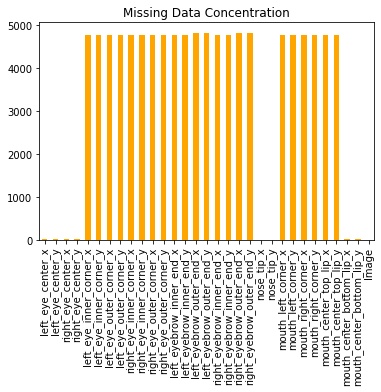
\includegraphics[scale=0.5]{missingData.png}
    \caption{Missing Data}
    \label{fig:my_label}
\end{figure}
    
    \item We have also used heat maps by Seaborn for finding the correlation between features as shown (Fig.3).

\begin{figure}[h!]
    \centering
    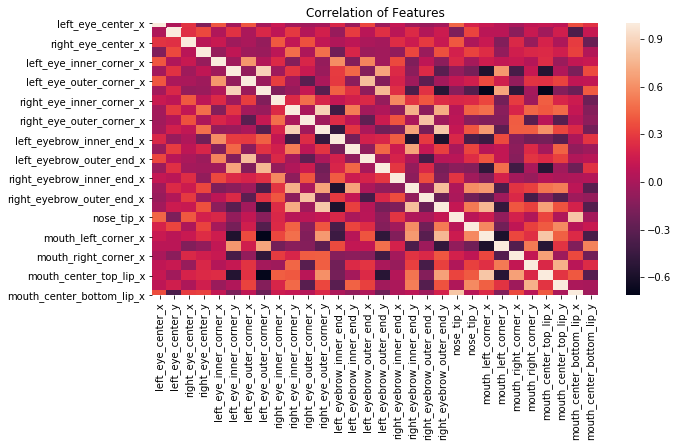
\includegraphics[scale=0.35]{correlationFeatures.png}
    \caption{Correlation of features}
    \label{fig:my_label}
\end{figure}
    
    \item Then we spilt the training into keypoints and images. Each row of keypoints data contains the (x, y) coordinates for 15 keypoints, while that of images data contains the row-ordered list of pixels.
\end{itemize}


\textbf{Visualizing the Input Image:} 

\begin{figure}[h!]
    \centering
    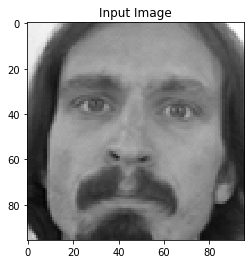
\includegraphics[scale=0.8]{sample.png}
    \caption{Input Image}
    \label{fig:my_label}
\end{figure}


\begin{itemize}
    \item Creating a numpy array of the pixel values in the image column of our training dataset. 
    
    \item Using matplotlib to plot the image from these pixel values.
    
    \item Using features such as left-eye-center-x, nose-tip-x, etc to plot keypoints on face images (Fig.5).

\begin{figure}[h!]
    \centering
    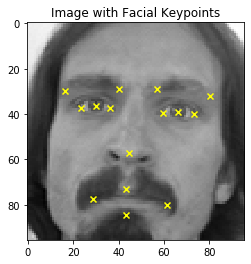
\includegraphics[scale=0.8]{sample+keypoints.png}
    \caption{Image with facial keypoints}
    \label{fig:my_label}
\end{figure}

    \item Formulating a gaussian function to create heatmaps of these facial keypoints (Fig.6).
    
    
    
    
\begin{figure}[h!]
    \centering
    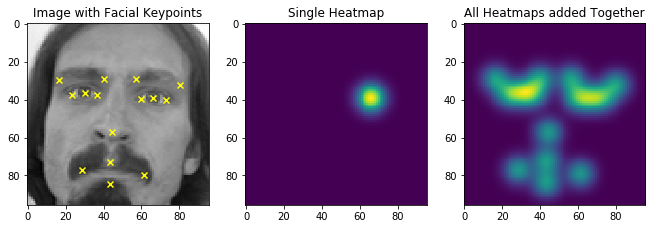
\includegraphics[scale=0.3]{sample+keypoints+heatmaps.png}
    \caption{Heatmaps of facial keypoints}
    \label{fig:my_label}
\end{figure}

\end{itemize}

\vspace{4mm}
\vfill



\textbf{Training:} 

Now that we have our processed data, we can train it using deep learning frameworks – Convolutional Neural Network and LeNet.

\textbf{Convolutional Neural Network -} In CNN, we have applied four convolutional layers.

The first step is to create convolution layer 1 in our network. The first element in the layer definition is Conv2d nn.Module method which creates a set of convolutional filters. There are three arguments used in this convolution layer; input channels, output channels and kernel size. The kernel-size argument is the size of the convolutional filter, in this case we want 5 x 5 sized convolutional filters, so the argument is 5. Then we have applied ReLU activation to this layer. The last element that is added in the layer definition is the max pooling operation. We then use batch normalization to limit covariate shift by normalizing the activations of each layer (transforming the inputs to be mean 0 and unit variance). This allows each layer to learn on a more stable distribution of inputs, and would thus accelerate the training of the network. We also specify a drop-out layer to avoid over-fitting in the model.

The second, third and fourth convolution layer are defined in the same way as the first layer. The only difference is the values for input channels and output channels depending on each layer. Applying ReLU, max pooling operating, batch normalization and dropout is done in the same way as the first layer.

The final output layer is a fully connected layer where the input from the other layers is flattened and sent so as the transform the output into the number of classes as desired by the network.

\textbf{LeNet -} In LeNet, we have applied two convolutional layers.

The first step is to create convolution layer 1 in our network. The first element in the layer definition is Conv2d nn.Module method. Three arguments used in this convolution layer are input channels, output channels and kernel size. In this case we want 5 x 5 sized convolutional filters, so the kernel size argument is 5. Then we have applied sigmoid activation to this layer. The last element that is added in the layer definition is the max pooling operation. 

Second convolution layer is defined in the similar way as the first one.

The final output layer is a fully connected layer.

With the above-mentioned deep network architectures, we have trained our model. 




\textbf{Evaluation:}

\begin{itemize}
    \item The models that we have created will now be applied to our training and testing data for evaluating the training and validation errors. Our goal is to minimize the error with subsequent iterations. 
    
    \item We have selected Adam to be our optimization algorithm since it is best suited for our deep learning frameworks. Our loss function is MSE (Mean Squared Error).
    
    \item Using the train test split function, we have split the target variable (Keypoints) from our Images. We are also creating a DataLoader in this function using torch.utils to load batches of our data for both Training and Validation data.
\end{itemize}

\section{RESULTS}

From our above trained model and predicting evaluations, we have plotted the graph of training and validation error for both CNN (Fig.7)and LeNet (Fig.8) as shown in the figure. 

\begin{figure}[h!]
    \centering
    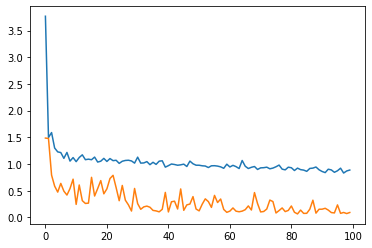
\includegraphics[scale=0.6]{cnn.png}
    \caption{Graph of Training and Validation error for CNN}
    \label{fig:my_label}
\end{figure}

\begin{figure}[h!]
    \centering
    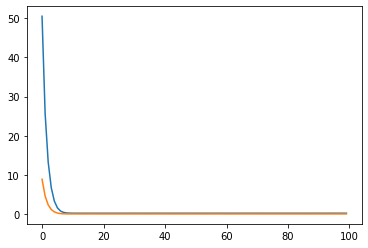
\includegraphics[scale=0.6]{LeNEt.png}
    \caption{Graph of Training and Validation error for LeNet}
    \label{fig:my_label}
\end{figure}
    
For better understanding of the results, we have visualized our outputs.

As we can see in Fig.9, we have plotted actual and predicted keypoints on the images.

\begin{figure}[h!]
    \centering
    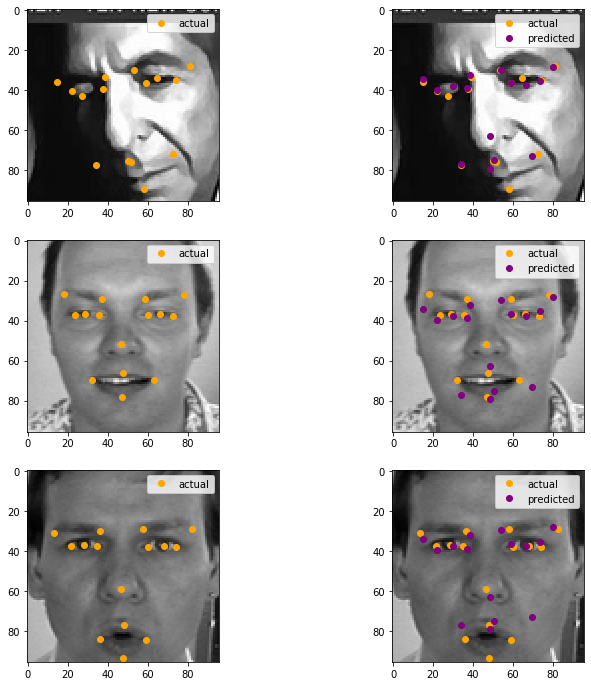
\includegraphics[scale=0.4]{ValidationImagesRealAndPredicted.png}
    \caption{Actual and Predicted Keypoints}
    \label{fig:my_label}
\end{figure}

Now we are going to use test dataset for predictions and visualizing test outputs as shown in Fig.10.

\begin{figure}[h!]
    \centering
    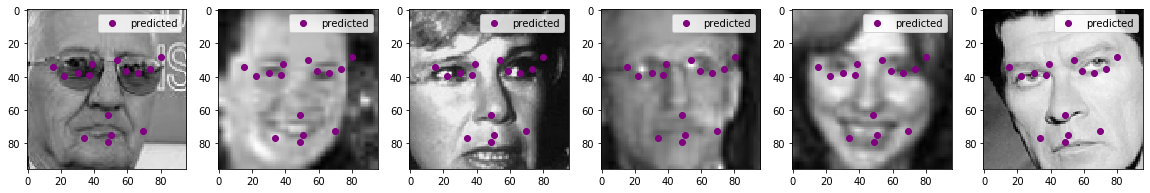
\includegraphics[scale=0.2]{testPredicted.png}
    \caption{Predicted keypoints for test dataset}
    \label{fig:my_label}
\end{figure}

Considering the results obtained for both networks we can observe how the LeNet5  network converges considerably faster in comparison with the random CNN of 4 layers. After the 15th epoch approximately the LeNet converges showing not improvement afterwards.

However in the case of the CNN, we can see how the model accuracy bounces around during the first 150 epochs, afterwards the model stabilizes the error and it slowly decreases it. Around the epoch 350 the validation error stops decreasing but the training error keeps decreasing, at this point we can stop the training other ways it may cause overfitting.

As conclusion, if we are looking for accuracy over speed then we will choose the CNN 4 layers model, but if what we are looking for is speed and we do not mind increasing the MSE then LeNet would be the choice. Note that the MSE reduction obtained by choosing the CNN 4 layers over the LeNet is from 0.0569 to 0.031

Now that we have completed everything, we must create a submission file.

Extending further with this implementation, we tried to take our own input image which is not necessarily a face image. We took an input image which contains a group of people (Fig.11). 

\begin{figure}[h!]
    \centering
    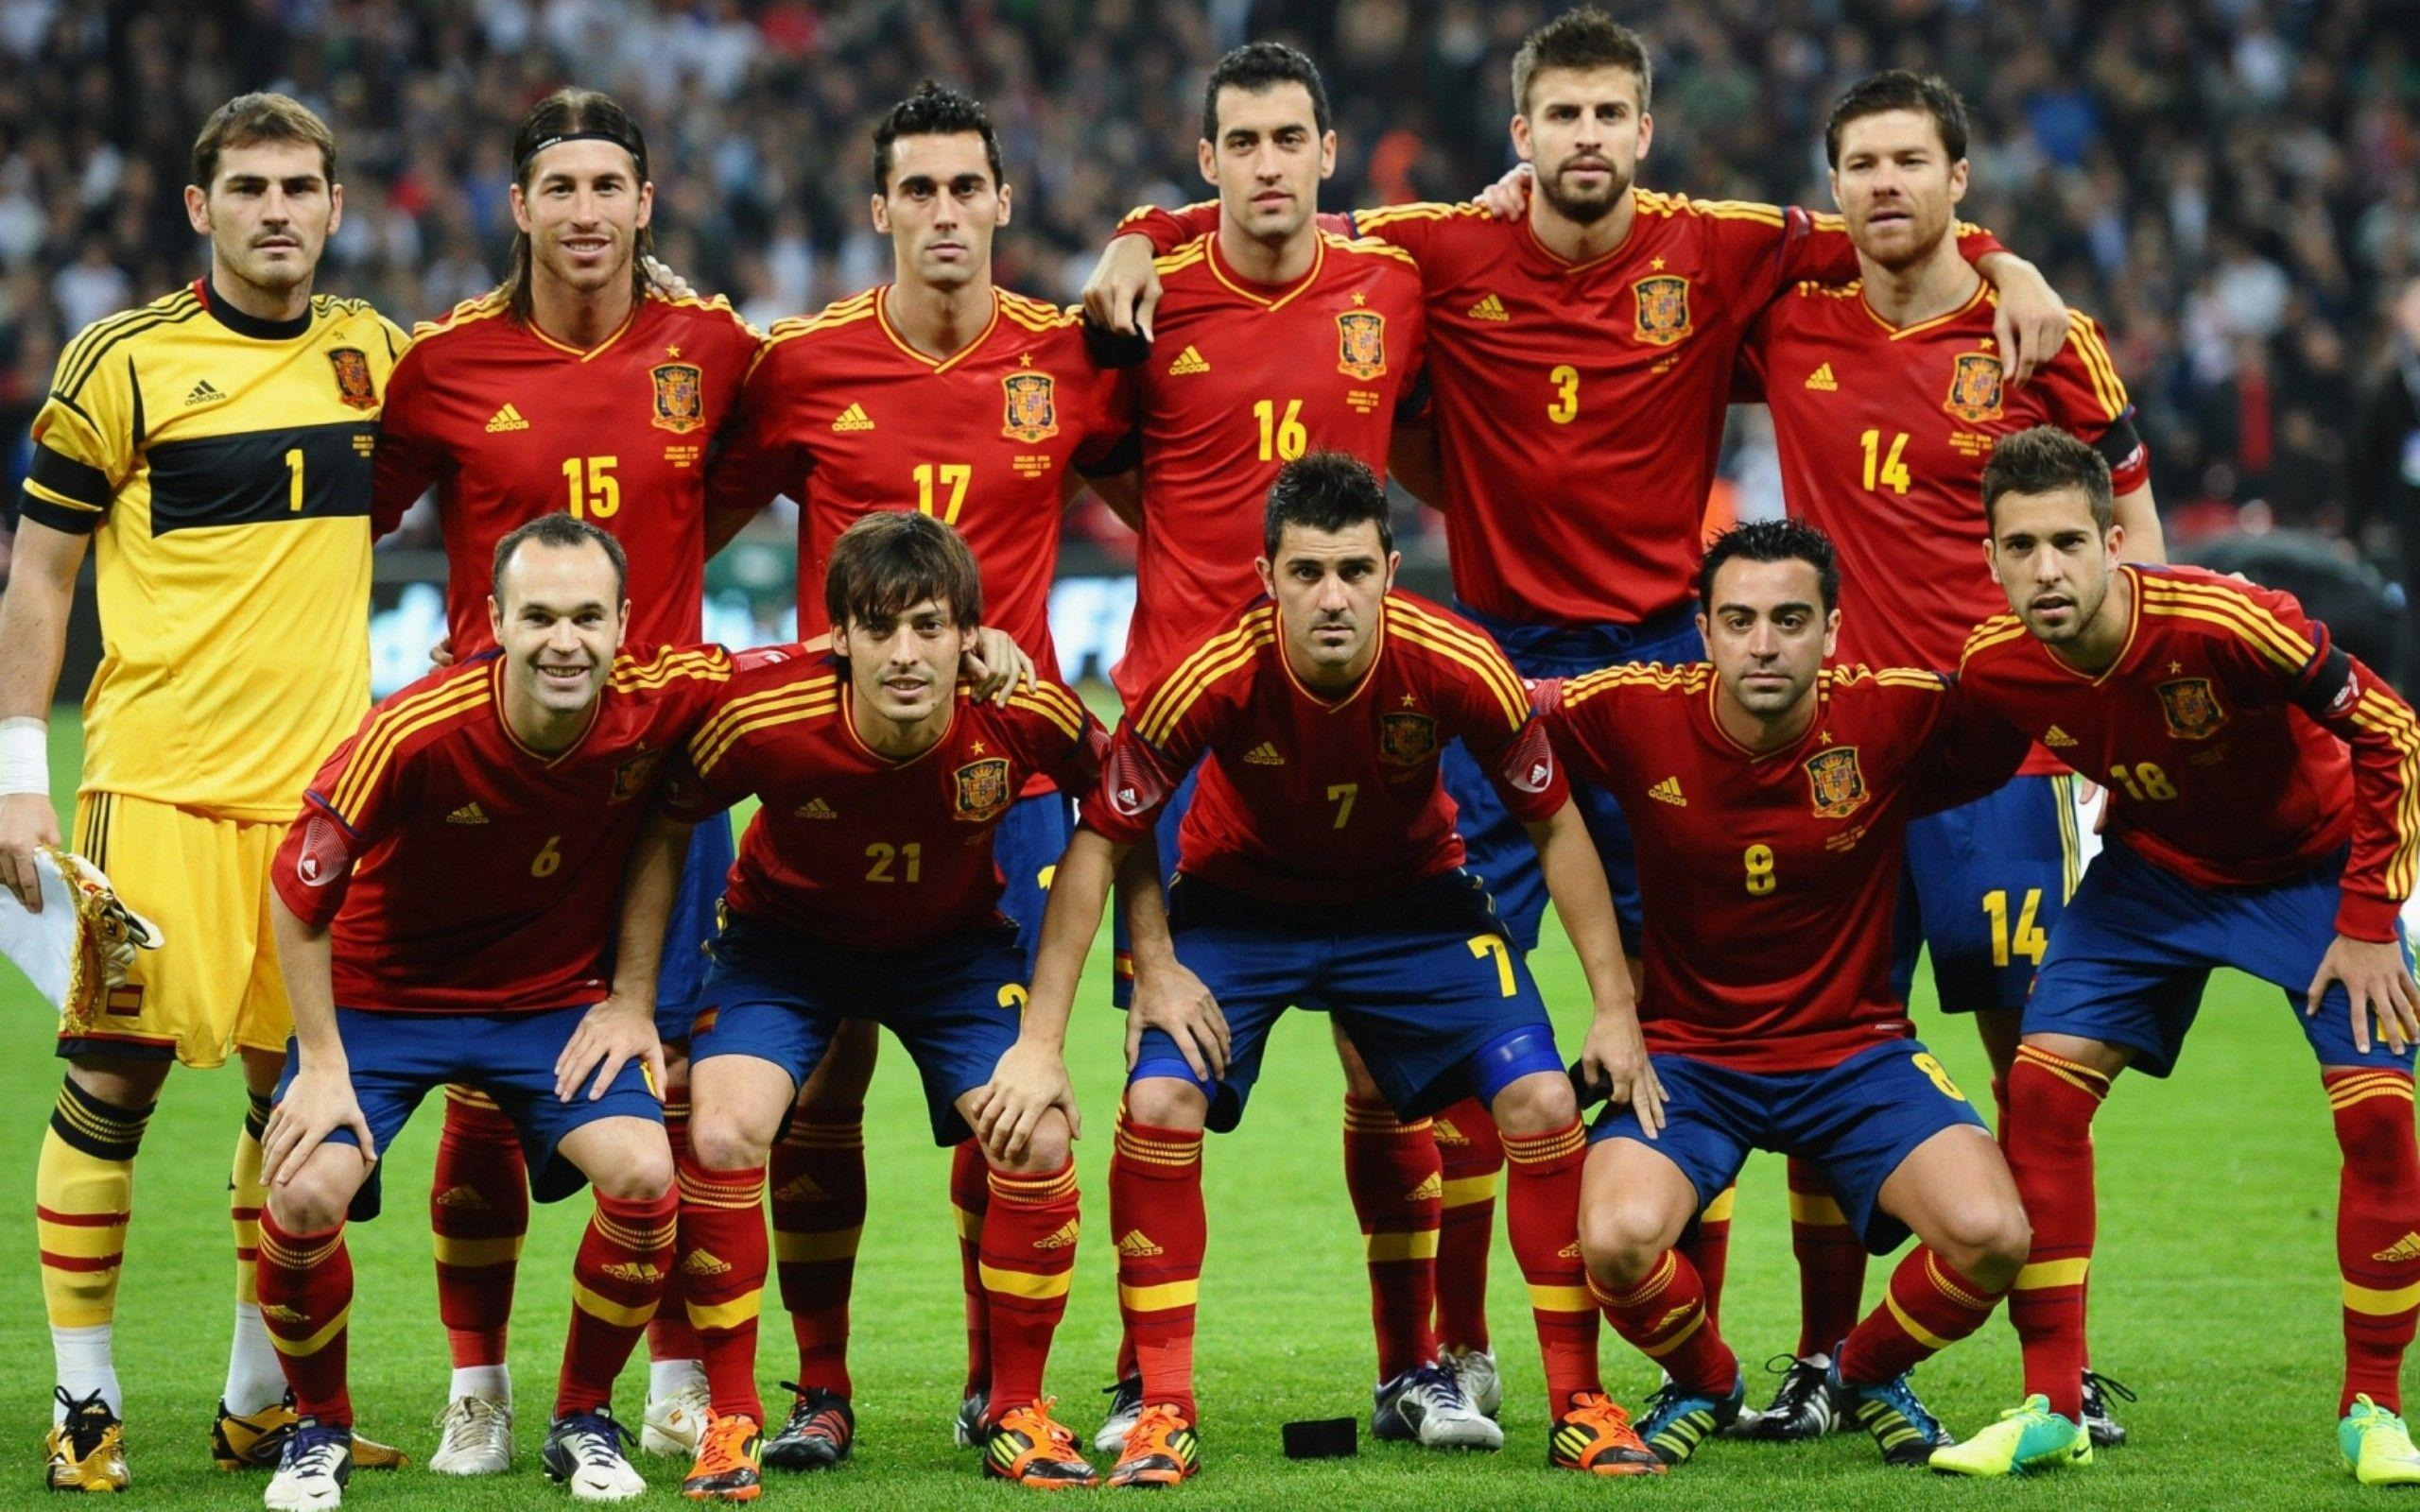
\includegraphics[scale=0.08]{FootballPlayers.jpg}
    \caption{Random input image}
    \label{fig:my_label}
\end{figure}

Haar cascade classifier is used for face detection in this image as shown in Fig.12. 

\begin{figure}[h!]
    \centering
    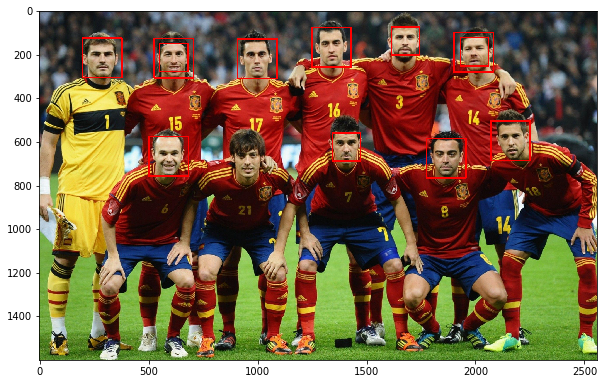
\includegraphics[scale=0.35]{original+faceboxes.png}
    \caption{Face Detection}
    \label{fig:my_label}
\end{figure}

Now we have detected the face images from our input image, we resized the face images so that it would fit our project requirements (Fig.13). 

\begin{figure}[h!]
    \centering
    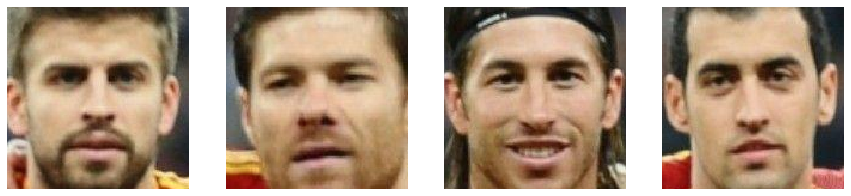
\includegraphics[scale=0.25]{new.png}
    \caption{Detected faces}
    \label{fig:my_label}
\end{figure}

Finally, we have applied our trained CNN and ResNet model to these detected face images. We successfully achieved facial keypoints detection of these images as shown in figure. So now we can use any image and locate keypoints on it (Fig.14).

\begin{figure}[h!]
    \centering
    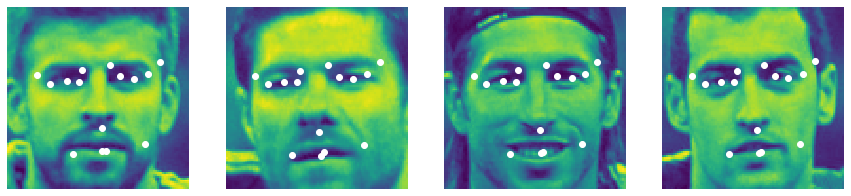
\includegraphics[scale=0.25]{newdots.png}
    \caption{Keypoints on detected faces}
    \label{fig:my_label}
\end{figure}




\section{CONCLUSION}

In this paper, we have focused on the task of detecting facial keypoints when given raw facial images. Specifically, for a given 96 x 96 image, we would predict 15 sets of (x, y) coordinates for facial keypoints. A deep structure, Convolutional Neural Network is successfully applied for Facial Key Points Detection problem. We further explored another deep model, LeNet to fit the requirements for detecting facial keypoints. Experiments which conducted on real-world Kaggle dataset have shown the effectiveness of deep structures. Comparing both the models, LeNet works better.

Extending further in this project, we have used different images containing a group of people rather than a single face. We have detected the faces of all the people from the images and successfully applied Convolutional Neural Network and LeNet i.e. our trained model to predict facial keypoints on those detected face images. Likewise, we can randomly pick any image with any number of people in it and apply our project to it.


\section{FUTURE SCOPE}

Given enough computation resources and time, CNN can be further modified by experimenting with different initialization schemes, different activation functions, different number of filters and kernel size, different number of layers, switching from LeNet to VGGNet, introducing Residual Networks, etc.  

    
Different image pre-processing approaches like histogram stretching, zero centering, etc. can be tried to check which approaches improve the model’s accuracy. 
 
    
Different resolution can greatly affect the results of the facial keypoints detection, thus what we can do is try to reduce the resolution of our given raw images to see the variance of the performance to further evaluate our model.




\section*{Acknowledgment}

It is with great satisfaction and achievement that we have completed this project and we would like to take this opportunity to acknowledge everyone who contributed towards our work. We express our sincere gratitude towards Prof.Sergul Aydore, for her guidance and support. We would also like to thank our teaching assistant Tianhao Zhu for his support. We are grateful for their cooperation and valuable suggestions.

\begin{thebibliography}{99}
    \bibitem{b1}D. Vukadinovic and M. Pantic. Fully automatic facial feature point detection using gabor feature based
    boosted classifiers. In Systems, Man and Cybernetics,
    2005 IEEE International Conference on, volume 2,
    pages 1692–1698. IEEE, 2005.
    
    \bibitem{b2}E.-J. Holden and R. Owens. Automatic facial point
    detection. In Proc. Asian Conf. Computer Vision, volume 2, page 2, 2002.
    
    \bibitem{b3}A. S. Mian, M. Bennamoun, and R. Owens. Keypoint
    detection and local feature matching for textured 3d
    face recognition. International Journal of Computer
    Vision, 79(1):1–12, 2008.
    
    \bibitem{b4}M. Valstar, B. Martinez, X. Binefa, and M. Pantic. Facial point detection using boosted regression
    and graph models. In Computer Vision and Pattern Recognition (CVPR), 2010 IEEE Conference on,
    pages 2729–2736. IEEE, 2010.
    
    \bibitem{b5}B. Martinez, M. F. Valstar, X. Binefa, and M. Pantic. Local evidence aggregation for regression-based
    facial point detection. Pattern Analysis and Machine
    Intelligence, IEEE Transactions on, 35(5):1149–1163,
    2013.
    
    \bibitem{b6}Y. Sun, X. Wang, and X. Tang. Deep convolutional
    network cascade for facial point detection. In Proceedings of the IEEE Conference on Computer Vision
    and Pattern Recognition, pages 3476–3483, 2013.
    
    \bibitem{b7}M. Haavisto et al. Deep generative models for facial keypoints detection. 2013.
    
    \bibitem{b8}Shenghao Shi, Facial Keypoints Detection, Research Gate,2017.
    
    \bibitem{b9}CNN Layers - PyTorch Deep Neural Network Architecture,
    "https://deeplizard.com/learn/video/IKOHHItzukk", 2018.
    
    \bibitem{b10} Q. Wang and J. Yang (2006). Eye Location and Eye State Detection in
    Facial Images with Unconstrained Background. Journal of Information and Computing Science, vol. 1(5), pp. 284-289.
    
    \bibitem{b11}A. Ng (2014). Lecture Notes for CS229 - Machine Learning. Stanford
    University.
    
    \bibitem{b12}K. He, X. Zhang, S. Ren and J. Sun, "Deep Residual Learning for Image
    Recognition," in Computer Vision and Pattern Recognition, 2015.
    
    \bibitem{b13}C. Szegedy, W. Liu, Y. Jia, P. Sermanet, S. Reed, D. Anguelov, D. Erhan,
    V. Vanhoucke and A. Rabinovich, "Going Deeper with Convolutions," in Computer Vision and Pattern Recognition, 2014.
    
    \bibitem{b14}K. Simoyan and A. Zisserman, "Very Deep Convolutional Networks
    for Large-scale Image Recognition," in International Conference on Learning Representation, 2015.
    
    \bibitem{b15}Y. LeCun, L. Bottou, Y. Bengio and P. Haffner, "Gradient-Based
    Learning Applied to Document Recognition," in Proceedings of the IEEE, 1998.
\end{thebibliography}
\vspace{12pt}
\color{red}


\end{document}

